%%%%%%%%%%%%%%%%%%%%%%%%%%%%%%%%%%%%%%%%%%%%%%%%%%%%%%
%%
%%           EE474 Hardware and Basic I/O
%%
%   % combined into notes pack
%
%\documentclass{article}
%\documentclass{seminar}
%
%\newpagestyle{BHstyle}{\sl U. of Washington \hfil EE 474 \hfil \thepage}{Hannaford \hfil \today}
%\pagestyle{headings}
%\slidepagestyle{BHstyle}
%\addtolength\oddsidemargin{3cm}
%\usepackage[T1]{fontenc}
%\usepackage[utf8]{inputenc}
%\usepackage[english]{babel}
%\usepackage{graphicx}
%\usepackage[pdftex,
%    pdftitle={ECE 474: Interrupts},
%    pdfauthor={Blake Hannaford, University of Washington},
%    pdflang={en-US},
%    pdfsubject={ECE 474 Embedded Microcomputer Systems},
%    pdfkeywords={embedded systems, microcontrollers, ECE 474},
%    hidelinks,
%    unicode]{hyperref}
%\usepackage{listings}
%
%
%\oddsidemargin 0in
%\evensidemargin 0in
%\textwidth 6.5in
%\textheight 8.7in
%\topmargin 0.2in
%
%
% 
%\linespread{1.0}
%
	%<*>
%\begin{document}
%\begin{slide}

%%%%** Section 1 
\section{Process Context}
%%%%** Section 1.1
\subsection{What is context?}
A process is sometimes called a task, subroutine or
program.  Process {\bf context} is all the information that
the process needs to keep track of its state.

\begin{description}
\item[Registers]   Temporary storage locations for a few
bytes.  Typical CPU has 8-64 registers.
\item[Program Counter] A special register which points to the
next instruction to be executed.
\item[Stack Pointer] Another special register which points to
the top (bottom) of a stack of data
\item[Processor Flags] Hardware bits in the CPU which detect
errors or arithmetic results.
\end{description}

Sometimes also called ``processor state''.

Example:  reading a book and the phone rings.

%\end{slide}
%\begin{slide}

%%%%** Section 1.2
\subsection{Context Switching}

When we call a subroutine (function) or when an
interrupt happens, we need to {\bf save} the current context
because we are starting a new one.

This happens a lot so it must be efficient.


\begin{itemize}
         \item After function completes, must know where to resume.
         \item New process can mess up information in old process.
        (i.e. what if they both use the same register?)
        \item Saving the context and restoring it is called
        {\bf context switching}.
\end{itemize}


%\end{slide}
%\begin{slide}

Procedure: To switch contexts from Process 1 to Process 2:
\begin{enumerate}
\item Control is passed from Proc1 to ``OSH"
\item OSH saves processor state from CPU registers(immediately!)
\item OSH finds stored state of Proc2 and restores it
into CPU registers.  IR is restored last.
\item CPU jumps to Proc1 code according to IR.
\end{enumerate}
{\bf OSH = Operating System or Hardware.}

%\end{slide}
%\begin{slide}

%%%%** Section 1.3
\subsection{Types of Context Switches}

\begin{itemize}
\item Subroutine Call. Either to user routine or to OS.
\item Interrupt.  Hardware initiated context switch.
\end{itemize}


%\end{slide}
%\begin{slide}

%%%%** Section 1.4
\subsection{Calls}

\begin{itemize}
\item User subroutine (e.g. {\tt sin($\theta$)}  ).  \\
  Main program context is saved, {\tt sin($\theta$)} routine is loaded.
\item System Calls Examples
        \begin{itemize}
        \item I/O such as write block of data to disk
        or apply a value to D/A converter.
        \item Process Control:  halt, wait (pend),
        start, kill, or unblock another process.
        \item Interprocess Communication:  pipes,
        mailboxes, semaphores.
        \item Return from Interrupt.
        \end{itemize}


\end{itemize}

%\end{slide}
%\begin{slide}

%%%%** Section 1.5
\subsection{The Stack}
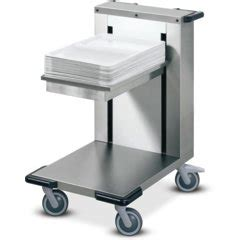
\includegraphics[width=2in]{misc_figs/traystack.png}\\
\noindent
Did your school cafeteria have one of these?\vspace{0.2in}

Problem:  How to allocate space for context storage. Consider
nesting of subroutine calls.
Solution: A stack is a data structure modeled on a spring-loaded cafeteria stack.

\begin{itemize}
        \item {\bf Push:} a piece of information on the stack.
        \item {\bf Pop: } a piece of information off of the stack.
        \item Always put/take info from current stack top.
\end{itemize}



Stacks are implemented with a {\bf Stack Pointer}.
 Enter the proper C code on the blank lines according	%<ch>
 to class discusion.	%<ch>

\begin{itemize}

% \item {\bf Push:} {\tt (*SP--) = piece\_of\_information}
 \item {\bf Push:} {\tt \_\_\_\_\_\_  =piece\_of\_information}	%<ch>
% \item {\bf Push:} {\tt *(SP--) =piece\_of\_information}

% \item {\bf Pop:}  {\tt SP++ ; piece\_of\_information = *SP }
 \item {\bf Pop:}  {\tt piece\_of\_information = \_\_\_\_\_\_ }	%<ch>
% \item {\bf Pop:}  {\tt SP++ ; piece\_of\_information = *SP }

        \item {\bf Initialize Stack:} {\tt SP = stack\_top}
        \item Stack grows down.
        \item Have to allocate space for maximum stack depth.
\end{itemize}


%\end{slide}
%\begin{slide}

%%%%** Section 1.6
\subsection{Subroutine Call}
How to call a subroutine (function in C).
(the compiler generates instructions to do all this
so you don't have to!)
\begin{enumerate}
        \item Push i argument {\it values} to stack: \\
% <s>                {\tt foreach {i} (*SP)-- = argument(i);}
                {\tt foreach {i} \_\_\_\_\_\_ = argument(i);}
% <n>                {\tt foreach {i} *(SP--) = argument(i);}
        \item Generate {\tt JSR} machine instruction.
        \begin{enumerate}
                \item Push machine registers onto stack.
                \item Load subroutine addr into PC
                \item execute next instruction (i.e. jump to
                *PC).
        \end{enumerate}
        \item Subroutine looks for arguments at {\tt
                *(SP - MACH\_REG\_SIZE) }
        \item When Subr. completes, execute {\tt RET} instruction.
        \begin{enumerate}
                \item Pop machine registers from stack.
                \item Clean up stack from function args:
                {\tt foreach {i} SP++;}
                \item Load old value into PC
                \item execute next instruction (i.e. jump to
                *PC).
        \end{enumerate}



\end{enumerate}

%%%%** Section 2 
\section{Interrupts}

An interrupt stops whatever instruction sequence is being executed by the processor and starts
some new code.  This happens in response to a specific hardware event event (the ``Interrupt") which 
could be internal or external.  The purpose of the new code is to immediately perform tasks 
specifically related to the event.   Let's look at some common terms used with interrupt programming.

\subsection{Interrupt Definitions}

{\bf Interrupt Service Routine (ISR):} When an interrupt is generated, some code, 
called an ISR, must be run immediately to “service” the interrupt.   ``Service"
means to perform tasks needed by the event that caused the interrupt.   For an 
extremely simple example, if a timer is causing regular clock interrupts, an ISR 
might just increment a variable called “time” and return.  A more advanced 
example would be a disk drive which earlier got a command to read data from a 
hardware disc sector.    After the sector read is completed, the drive generates 
an interrupt, and the ISR must grab the data from the drive and put it into the 
right place in memory. 

{\bf Enabling interrupts:  } Just like when you concentrate on some reading or 
writing task, interruptions are costly for the CPU.  Furthermore, if there is no 
ISR defined for the interrupt, then acting on that interrupt could hang (freeze) 
the system.   Therefore there are bits controlled by software that enable or 
disable interrupts from hardware signals.   By default all the interrupts are 
disabled.    In addition to enabling individual interrupts, the CPU has bits 
that can globally enable or disable all interrupts.

{\bf Internal Interrupts:} Interrupts from components inside the computer itself such as timer/counters. 

{\bf External interrupts: } Interrupts from components outside the CPU such as a digital input bit, a network interface, or an SSD.

{\bf Interrupt Priorities:}   Interrupts can interrupt ISRs(!)  ... or not!    You might have one interrupt which is a very time-critical control function, and a plane will crash if this ISR does not execute correctly in 2milliseconds.   You might also have another ISR that updates a log file.   The first ISR is therefore a much higher priority than a log-file update.   Yes, we need to guarantee that the log file gets updated, but the speed does not matter.    Most processors group the available interrupts into priority levels such that lower priority interrupts have to wait until there are no running ISRs of higher priority. 

{\bf Interrupt Vectors: }    A powerful computer system could have many different interrupts that are enabled at a given time.   A simple example would be a Network-Attached-Storage (NAS) device which is basically a computer with a bunch of disk drives (or SSDs) attached to it to be a file server.    If there are four drives attached to the NAS, each one needs a separate interrupt so that they can operate simultaneously.   The way to implement this is for each hardware interrupt mechanism to have a pointer to a software ISR function.    The address of the ISR for each interrupt is the “Interrupt Vector”.  

{\bf Interrupt Vector Table:}  This is a hardware-specific region of memory that is specially set aside (and hardware-defined) to hold an interrupt vector for each hardware interrupt the processor can support.   If the interrupt is not enabled then it doesn’t matter what is in the table, but for every enabled interrupt, there must be a valid pointer to a function that can run and return. 
 

Types of inputs that can cause an interrupt:
\begin{itemize}
        \item User pushes a button or moves a mouse.
        \item Packet arrives on network interface.
        \item A sensor detects an event.
        \item Disk drive
 completes an operation and has a bunch of data ready for CPU.	%<chn>
        \item A clock
 can be programmed to set up interupts at regular intervals.	%<chn>
        \item A hardware timer
 can count clock pulses and generate an interrupt when it gets to zero.	%<chn>
        \item A thermostat
 indicates that a temperature setpoint is reached.	%<chn>
\end{itemize}


\paragraph{Connections}

Interupts are logic signals physically wired to the CPU
(or interrupt processor peripheral).	%<chn>

There are various schemes for wiring multiple interrupts:

\paragraph{Priority}

\begin{itemize}
        \item 7 lines leading into CPU.
        \item peripherals can pull one line low
 for example using open collector ``wired OR''.	%<chn>
        \item A small address bus identifies the specific
        interrupt within a line.
        \item Lines are ranked by priority
 e.g. ISR for Line 0 cannot be interrupted by any other interrupt,	%<chn>
ISR for Line 6 can be interrupted by ANY other interrupt.	%<chn>
\end{itemize}

\paragraph{Interrupt Vectors}

Each interupt has a specific code number which is applied to
the processor interrupt address bits (maybe 8bits).

CPU has a specific hard-wired memory address called the
{\bf interrupt vector table.}    The interrupt vector
table is an array of function pointers.  The functions
they point to are called
{\bf interrupt service routines, ISRs}.

\paragraph{Typical Interupt Vector Table}
{\tt
\begin{tabular}{|r|r|}
\hline
Memory Addr             &       Contents \\ \hline

1000                    &       isr\_0()  \\ \hline
1002                    &       isr\_1()  \\ \hline
1004                    &       isr\_2()  \\ \hline
1006                    &       isr\_3()  \\ \hline
...                     &       ...       \\ \hline
1100                    &       isr\_N()  \\ \hline

\end{tabular}
}

\paragraph{Meaning of ISRs}

Each hardware device is hooked up to a specific interrupt vector
table address.  We need to write each ISR to handle the proper
device.

%%%%** Section 2.1
\subsection{ISRs}

\paragraph{Servicing an interrupt}

\paragraph{Hardware Level}

 The hardware does the following steps when an interupt	%<chn>
is detected:	%<chn>

% Upon hardware interrupt:
\begin{enumerate}
        \item Push processor context onto stack.
        \item Load appropriate address from IVT into
        program counter (PC).
        \item jump to *PC.
\end{enumerate}

\paragraph{Software Level}

 The ISR is now in control.  The ISR must do the	%<chn>
 following.	%<chn>

\begin{enumerate}
        \item (There are no arguments)
        \item block (``mask'') all other interrupts if necessary
        \item ``service'' the device.
        \item unmask other interrupts
        \item  Execute a return from interrupt instruction
\end{enumerate}

\paragraph{Hardware Level}

Now the hardware takes over again to clean up the interrupt.	%<chn>

\begin{enumerate}
        \item Pop processor context from the stack.
        \item Last item is PC
        \item continue whatever was being done when interrupt
        occured.
\end{enumerate}


%\end{slide}
%\begin{slide}

%%%%** Section 2.2
\subsection{ISR Programming}

 Some tips for successful ISR programming	%<chn>

\paragraph{Problems with ISRs}
\begin{itemize}
        \item ISRs are virtually impossible to debug!
        \item The debugger uses ``software interrupts'' to handle
        tricks like breakpoints and single stepping.
        \item thus even correct ISRs will break the debugger OR
        \item the debugger will break your ISRs
        \item ISRs take over the processor -- even pre-emptive
        schedulers.
        \item ISRs can easily mess up other processes if they

                \begin{itemize}
                \item write in wrong global variables
                \item take up a lot of CPU time
                \item play around with the stack
                \end{itemize}
\end{itemize}


%\end{slide}
%\begin{slide}

\paragraph{ISR Solutions}


\begin{itemize}
        \item Keep your ISRs  {\it small, simple, \& quick }
        \item No loops inside ISR's
        \item No complex logic (no nested {\tt if}'s )
        \item Don't do unrelated I/O in the ISR (for example,
        no {\tt printf("ISR message");}).
        \item Guidelines: Max: 1/2 page of C, 1 page of ASM
        \item Do not trust / use debugger.
        \item Do absolute minimum of stuff in ISR, do the
        rest in a regular task.
        \item Check and recheck your use of interrupt masking
        and how you save and restore the context.

\end{itemize}


%\end{slide}
%\begin{slide}
%%%%** Section 3 
\section{Real Time Control }

%%%%** Section 3.1
\subsection{Basic Task}
Map inputs to outputs (through a control law) at
{\it regular } time intervals.


%\end{slide}
%\begin{slide}

\begin{verbatim}
\% Initialization
set_up(timer0);
set_up(input,output);

\% endless control loop
while(1)
        {
        wait(timer0);
        x=read(input);
        y=control_function(x);
        output(y,output);
        }
\end{verbatim}

%\end{slide}
%\begin{slide}

%%%%** Section 3.2
\subsection{Timing}
Different ways to ensure regular time sampling.


\begin{itemize}
        \item While loop + Interrupt
        \begin{itemize}
                \item ``main" program is {\tt while(1);}
                \item Timer is set up for regular interrupts
                every {\tt T} seconds.
                \item ISR is I/O and control law: \\
                {\tt x=read(input); \\
                y=control\_function(x);  \\
                output(y,output); \\
                return();}
        \end{itemize}
%\end{itemize}

%\end{slide}
%\begin{slide}

%\begin{itemize}
        \item  ``spin-lock'': \\
         {\tt wait(timer0) $\to$ while(timer0 == 0) ;}
        \item  OS Call:   \\
        {\tt wait(event)} \\
        return control to OS until {\bf event} occurs.  {\bf event} is timer0.
\end{itemize}




%\end{slide}

%\end{document}
